\documentclass[12pt]{article}
\usepackage[english]{babel}
\usepackage[utf8]{inputenc}
\usepackage{graphicx}
% \usepackage{float}
\graphicspath{{images/}}
\usepackage[a4paper,width=170mm,top=20mm,bottom=25mm,bindingoffset=6mm]{geometry}
\usepackage{fancyhdr}
\usepackage{caption}
\usepackage{subfigure}
\usepackage{booktabs}
\usepackage{hyperref}
\usepackage[title, titletoc]{appendix}

\newcommand{\Florin}[1]{\textcolor{blue}{Florin: #1}}

\usepackage{amsmath}
\usepackage{bm}
\hypersetup{
    colorlinks=true,
    linkcolor=blue,
    filecolor=magenta,      
    urlcolor=cyan,
}
\urlstyle{same}
% \usepackage{natbib}
\bibliographystyle{unsrt}

\usepackage{floatrow}
\usepackage{multirow, makecell}
\usepackage{hhline}
\usepackage{array, booktabs}
\usepackage[svgnames]{xcolor} 
\usepackage{mathtools}
\usepackage{longtable}
\usepackage{indentfirst}


\usepackage{listings}
\usepackage{xcolor}

\pagestyle{fancy}
\fancyhf{}



\lhead{\color{Grey} 02450 Introduction to Machine Learning and Data Mining}
% \fancyfoot{}
% \fancyfoot[R]{\thepage}
% \fancyfoot[L]{\today}

% \pagestyle{fancy}
\lfoot{\color{Grey} Group 43}  
\rfoot{\color{Grey} Report 1}
\cfoot{\color{Grey} \thepage}

\renewcommand{\headrulewidth}{0.4pt}
\renewcommand{\footrulewidth}{0.4pt}
\setlength{\headheight}{14.5pt}

\title{
    
    {
\includegraphics[width=0.4\textwidth]{dtu_logo.png}}\\
    \vspace{1.5cm}
    \hrule 
    \vspace{1cm}
    \large 02450 Introduction to Machine Learning and Data Mining \\ 
    \vspace{1cm}
    \textbf{Report 1} \\
    \text Data: Feature extraction, and visualization
    \vspace{1cm} 
    \hrule
    \vspace{9cm}
}


\author{\\\textbf{Group 43} \\ Florin Mazilu (s222696) \\ Mihai-Valentin Andrei (s222695)\\Cristiana Lazar (s222698)}
\vspace{1cm}


\date{ October 2022}
 

 



\definecolor{codegreen}{rgb}{0,0.6,0}
\definecolor{codegray}{rgb}{0.5,0.5,0.5}
\definecolor{codepurple}{rgb}{0.58,0,0.82}
\definecolor{backcolour}{rgb}{0.95,0.95,0.92}

\lstdefinestyle{mystyle}{
    backgroundcolor=\color{backcolour},   
    commentstyle=\color{codegreen},
    keywordstyle=\color{magenta},
    numberstyle=\tiny\color{codegray},
    stringstyle=\color{codepurple},
    basicstyle=\ttfamily\footnotesize,
    breakatwhitespace=false,         
    breaklines=true,                 
    captionpos=b,                    
    keepspaces=true,                 
    numbers=left,                    
    numbersep=5pt,                  
    showspaces=false,                
    showstringspaces=false,
    showtabs=false,                  
    tabsize=2
}

\lstset{style=mystyle}




\newcommand{\ruijie}[1]{\textbf{\textcolor{red}{#1}}}

\newcommand{\ruixin}[1]{\textbf{\textcolor{blue}{#1}}}

\usepackage[font={small}]{caption}
\usepackage{color}




\makeatletter
\newcommand*{\rom}[1]{\expandafter\@slowromancap\romannumeral #1@}
\makeatother


\begin{document}

\maketitle


\begin{table}[H]
\begin{tabular}{|l|c|c|c|c|c|}
\hline
Student & Problems & Section 2 & Section 3 & Section 4 & Section 5 \\ \hline
s222696 & 33.33\% & 20\% & 30\% & 16.66\% & 66.66\% \\ \hline
s222695 & 33.33\% & 50\% & 40\% & 26.66\% & 16.66\% \\ \hline
s222698 & 33.33\% & 30\% & 30\% & 56.66\% & 16.66\% \\ \hline
\end{tabular}
\caption{Contribution of each group member.}
\label{table:1}
\end{table}
\tableofcontents
\listoffigures
\listoftables
\newpage
\section{Problems}
\begin{enumerate}
  \item \textbf{Question 1. Spring 2019 question 1} \\
  Option C, since there are only two attributes ordinal, Time of day - because the time is coded as a 30-minute interval, and Congestion level - because we have a degree of comparison between low congestion and high congestion, and the other attributes are ratio.
  \item \textbf{Question 2. Spring 2019 question 2} \\
  Option A. We can see this by computing the $d_{\infty}(x_{14}, x_{18})$:
  \begin{equation*}
      d_{\infty}(x_{14}, x_{18}) = \max(|26 - 19|, |0 - 0|, |2 - 0|, \dots, |0 - 0|) = 7
  \end{equation*}
  \item \textbf{Question 3. Spring 2019 question 3} \\
  Option A.
  The var explained by the first four principal components is 
  \begin{equation*}
    \frac{(13.9)^2 + (12.47)^2 + (11.48)^2 + (10.03)^2}{(13.9)^2 + (12.47)^2 + (11.48)^2 + (10.03)^2 + (9.45)^2} = \frac{581.1022}{670.4047}=0.866
  \end{equation*}
  \item \textbf{Question 4. Spring 2019 question 4} \\
  Option D.
For PCA2, \textit{Time of Day} has a negative coefficient, whereas \textit{Broken Truck}, \textit{Accident victim} and \textit{Defects} have a positive coefficient. Therefore, a low value for a negative coefficient and high values for positive coefficients will result in a positive value of the projection onto the second principal component.
  \item \textbf{Question 5. Spring 2019 question 14} \\
  Option A. The term-document matrix corresponding to the 2 text documents is shown in Table \ref{table:5} below:
  \begin{table}[H]
\begin{tabular}{|c|c|c|c|c|c|c|c|c|c|c|c|c|c|}
\hline
 & the & bag & of & words & repres. & becomes & less & parsim. & if & we & do & not & stem \\ \hline
s1 & 1 & 1 & 1 & 1 & 1 & 1 & 1 & 1 & 0 & 0 & 0 & 0 & 0 \\
s2 & 1 & 0 & 0 & 1 & 0 & 0 & 0 & 0 & 1 & 1 & 1 & 1 & 1 \\
\hline
\end{tabular}
\caption{Term-document matrix}
\label{table:5}
\end{table}
The Table \ref{table:5} we conclude that: \begin{equation*} f_{11} = 2 \end{equation*} and \begin{equation*} f_{11} + f_{10} + f_{01} = 13 \end{equation*}
In conclusion:
\begin{equation*} J(s1, s2) = \frac{f_{11}}{f_{11} + f_{10} + f_{01}} = \frac{2}{13}=0.153846\end{equation*}
  \item \textbf{Question 6. Spring 2019 question 27} \\
  Option B. We need to compute $p(\hat{x}_2 = 0| y = 2)$, thus we will look in the given table at the column where $y = 2$. Furthermore, $\hat{x}_7$ can be either $0$ or $1$, but $\hat{X}_2$ has to be $0$, so we only take into account the first two columns of the table. So:
  \begin{equation*}
      p(\hat{x}_2 = 0| y = 2) = p(\hat{x}_2 = 0, \hat{x}_7 = 0| y = 2) + p(\hat{x}_2 = 0, \hat{x}_7 = 1| y = 2) = 0.81 + 0.03 = 0.84
  \end{equation*}
\end{enumerate}
\clearpage
\setcounter{page}{1}

\section{Data set description}
The data we are working with is part of a \textit{Glass Identification} dataset, used to classify glass fragments into multiple types considering the chemical composition of the oxide. 
The number of instances in the original dataset was 214, but we are working with 163 observations from the main 2 glass classes (more in section \ref{PCA}). 

The dataset was downloaded from the UCI Machine Learning Repository\cite{data_set_source}. The data was donated in 1987 by Vina Spiehler a Ph.D. from DABFT (Diplomate of the American Board of Forensic Toxicologists). Vina initially used the data about the classification of types of glass as part of criminological investigation research, given that the glass left at the scene of a crime can be used as evidence if correctly classified.
\subsection{Previous analysis of the data}
In their article “Rule induction in forensic science”\cite{rule_induction_article}, Ian W. Evett and E.J. Spiehler build on the fact that scientists can determine the origin of a small glass fragment found at a crime scene as part of the forensic examination. They were using a new rule induction package called BEAGLE (Bionic Evolutionary Algorithm Generating Logical Expressions) that requires a database as input and classifies the results. 

The goal of the article is to compare the performance of this system to conventional statistical techniques (discriminant analysis and nearest neighbour). They conclude that BEAGLE was the best performer with an error rate of only 0.6\% when classifying the glass data.
\subsection{Our analysis objectives}
As a first step in our own analysis of the data, we want to investigate if the data is indeed correlated, in what way the different attributes are connected and whether the given attribute values are enough to predict the type class.

For the  \textit{classification task}, we are going to predict the Type of Glass class based on the refractive index and all 8 of the percentages for the chemical composition of the material (especially the percentages of magnesium and aluminum). The classification should be realized without much difficulty given the equal class distribution of observations (87 float-processed windows and 76 non-float-processed windows) and the clear correlation between the type and the attributes observed in section \ref{statistics}.

In our \textit{regression}, we are considering predicting the value for the percentage of calcium in the glass composition. This should be achievable given the strong correlation between calcium and the refractive index and calcium and magnesium percentage (Fig \ref{fig:correlation_matrix}).

\section{Attributes description}
\subsection{Classification of the attributes}

\begin{table}[H]
\begin{tabular}{|l|c|c|c|c|c|}
\hline
No. & Attribute name & Abbrev. 2 & Discrete/continuous & Type of attribute \\ \hline
$x_1$ & Refractive index & RI & continuous & interval \\ 
$x_2$ & Percentage of Sodium & Na & continuous & ratio \\ 
$x_3$ & Percentage of Magnesium & Mg & continuous & ratio \\ 
$x_4$ & Percentage of Aluminum & Al & continuous & ratio \\ 
$x_5$ & Percentage of Silicon & Si & continuous & ratio \\ 
$x_6$ & Percentage of Potassium & K & continuous & ratio \\ 
$x_7$ & Percentage of Calcium & Ca & continuous & ratio \\ 
$x_8$ & Percentage of Barium & Ba & continuous & ratio \\ 
$x_9$ & Percentage of Iron & Fe & continuous & ratio \\ \hline
$x_{10}$ & Type of Glass & type & binary & nominal \\ \hline
\end{tabular}
\caption{Types of attributes for the Glass data set comprised of N = 163 observations and M = 10 features}
\label{table:2}
\end{table}
Table \ref{table:2} above provides a summary of the attributes of the data and their types.

The first attribute, $ x_{1} $, is the Refractive index of the glass, which indicates the light bending ability of the glass medium. It is the most important property of the glass because it varies considerably from one glass object to another\cite{rule_induction_article}. It is a floating-point number with 5 given decimals and ranges from 1.5121 to 1.5339 as seen in table \ref{table:3}. Therefore, it is a \textit{continuous} feature. It is also an \textit{interval} attribute, because it is ordered and the relative magnitude of the variable has a physical meaning (the difference in how much the path of light is refracted when entering the glass). The value ‘0’ holds no meaning, as the value ‘1’ is by definition the smallest possible refractive index, the one for vacuum\cite{refractive_index}. 
 
The next 8 attributes all represent the weight percentage of specific chemical elements in the composition of the corresponding oxide. The 8 percentages are exhaustive in relation to the composition of the specific glass. These values are floating-point numbers with 2 decimals, ranging from 0.00 to 74.45. They represent \textit{continuous} attributes. Additionally, the values can be ranked, the distance/difference between them can be measured and value ‘0’ corresponds to the complete absence of the specific chemical element from the glass composition. Therefore, they are all \textit{ratio} features.

The Type of Glass is the class label that will be predicted during the classification task. It consists of a small countable set of values, which makes it a \textit{discrete} feature. Originally the dataset included 7 possible values for the type of glass, which were unevenly distributed as seen in table \ref{table:4}. As a pre-processing step described in section \ref{PCA}, we decided to remove some of the initial observations which represented infrequent glass types and we were left with 2 main classes: float-processed window glass and non-float-processed window glass.
Float-processed here refers to the modern process of floating molten glass on a bed of molten metal in order to give the sheet of glass uniform thickness and very flat surfaces. Having now only 2 possible values, this attribute can be further considered a \textit{binary} feature. Because the values reflect categories of observations, which cannot be ranked or measured, the Type of Glass is a \textit{nominal} attribute.

The original dataset also included an index attribute, which we decided to also remove during the pre-processing phase as it was deemed to be mostly irrelevant.

The dataset does not contain any data issues. There were no missing values or any corrupted data. Additionally, the values for attributes $ x_{2}-x_{9} $ always add up to approximately 100\% which further validates the correctness of the data.


\subsection{Summary statistics} \label{statistics}
\begin{table}[H]
\begin{tabular}{llllllllll}
         & RI     & Na      & Mg      & Al     & Si      & K      & Ca     & Ba     & Fe     \\
mean     & 1.5185 & 13.2017 & 3.2949  & 1.2816 & 72.5869 & 0.4774 & 8.9246 & 0.0298 & 0.0676 \\
std      & 0.0030 & 0.5883  & 0.8877  & 0.3237 & 0.6411  & 0.2187 & 1.3726 & 0.2535 & 0.0995 \\
median   & 1.5177 & 13.21   & 3.54    & 1.29   & 72.7    & 0.57   & 5.55   & 0      & 0      \\
min      & 1.5121 & 10.73   & 0       & 0.29   & 69.81   & 0      & 7.08   & 0      & 0      \\
max      & 1.5339 & 14.86   & 4.49    & 2.12   & 74.45   & 1.1    & 16.19  & 3.15   & 0.37   \\
range    & 0.0217 & 4.13    & 4.49    & 1.83   & 4.64    & 1.1    & 9.11   & 3.15   & 0.37   \\
corrcoef & 0.007  & -0.1434 & -0.3092 & 0.3663 & 0.0162  & 0.1867 & 0.1017 & 0.0756 & 0.1142
\end{tabular}
\caption{Summary statistics}
\label{table:3}
\end{table}
The table \ref{table:3} shows the summary statistics of the data set. These statistics gave us insights into the correctness of the samples. As can be seen, the RI attribute, which represents the refractive index, has a mean equal to 1.518 (and has a low value for the standard deviation), which is equal to the average refractive index of the glass. By comparing the concentration with the expected values\cite{glass_composition}, we saw that the range of values was within approximate limits. For example, the approximate limits, in the case of typical float glass, for $Na_2O$ are 9-15 mol\%, and in our data set, the minimum and maximum values are 10.73 and 14.86. For a float-processed glass, the mole percent $Ba$ should be 0, while for a non-float-processed glass the approximate limits are 0.5-6.5 mol\%. Therefore, the values in the data set reflect reality.

In order to provide information about correlation, we plotted the correlation matrix (Fig. \ref{fig:correlation_matrix}). We noticed that the refractive index, RI, is strongly positively correlated with Ca and slightly negatively correlated with Si. Also, Ca is strongly negatively correlated with Mg. In spite of that, the most important observation is the correlation between the type and the attributes. In this case, the type correlates with Mg and Al attributes (negatively and, respective, positively). These observations are relevant in the classification context. Therefore we expect that the classification should be easily realized.
\begin{figure}[H]
        \centering
    	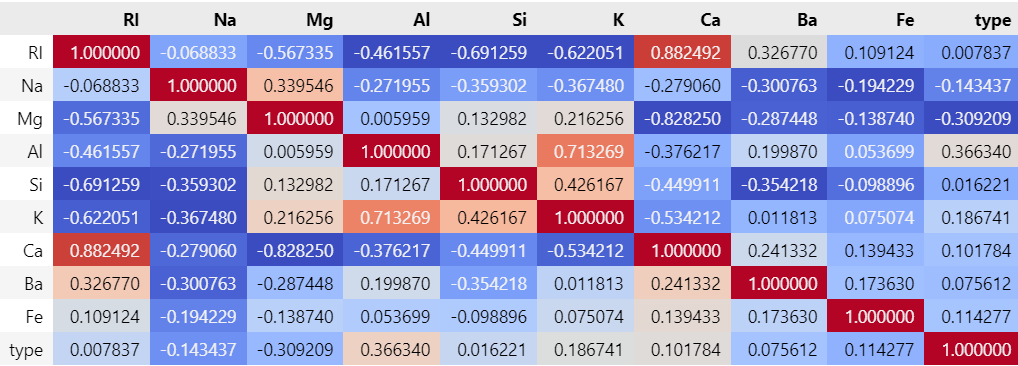
\includegraphics[width=\linewidth]{image/correlation_matrix.png}
    	\caption{The correlation between each attribute.}
    	\label{fig:correlation_matrix}
\end{figure}

\section{Data visualization}
To supplement our summary tables we included individual visualization of each of the attributes. 
    \begin{figure}[H]
        \centering
    	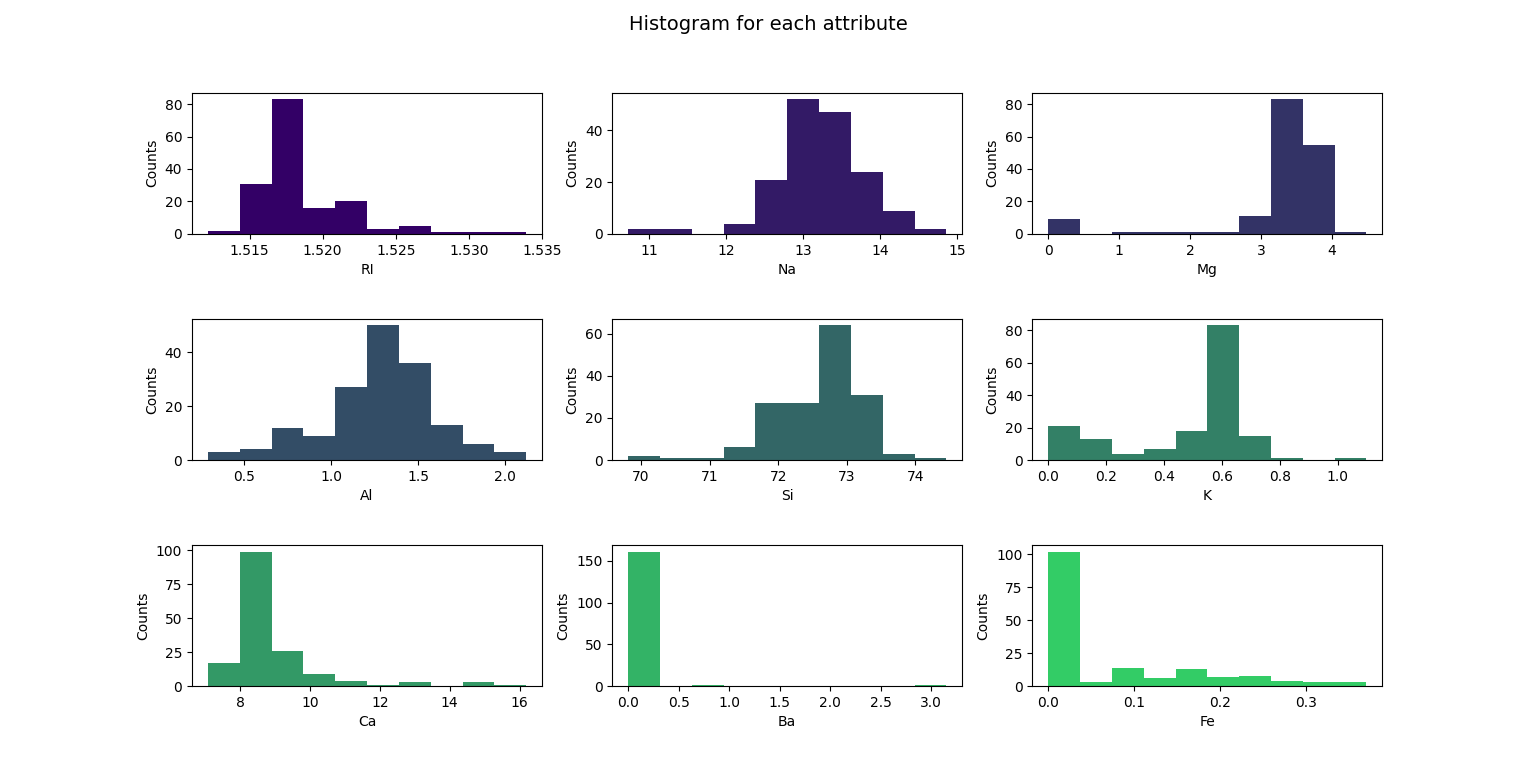
\includegraphics[width=\linewidth]{image/histogram_for_each_attribute.png}
    	\caption{The attributes' distribution is visualized using a histogram.}
    	\label{fig:histogram}
    \end{figure}
    
    
Analyzing the histogram from Fig. \ref{fig:histogram}, $Ba$ attribute we noticed that almost all values are between 0.0 and 1.0, and just a sole sample has $Ba$ concentration equal to 3.0. By plotting the box-plot Fig. \ref{fig:box_plot}, we could easily conclude that the sample must be an outlier. Nevertheless, by creating a different box-plot for each class Fig. \ref{fig:box_plot_float} and Fig. \ref{fig:box_plot_non_float}, we noticed that the sample is classified as non-float glass. Knowing that the approximate limits for the concentration of Ba in a not-float glass are 0.5-6.5\% mol \cite{glass_composition} led us to the conclusion that the sample is not an outlier.
    
    \begin{figure}[H]
        \centering
    	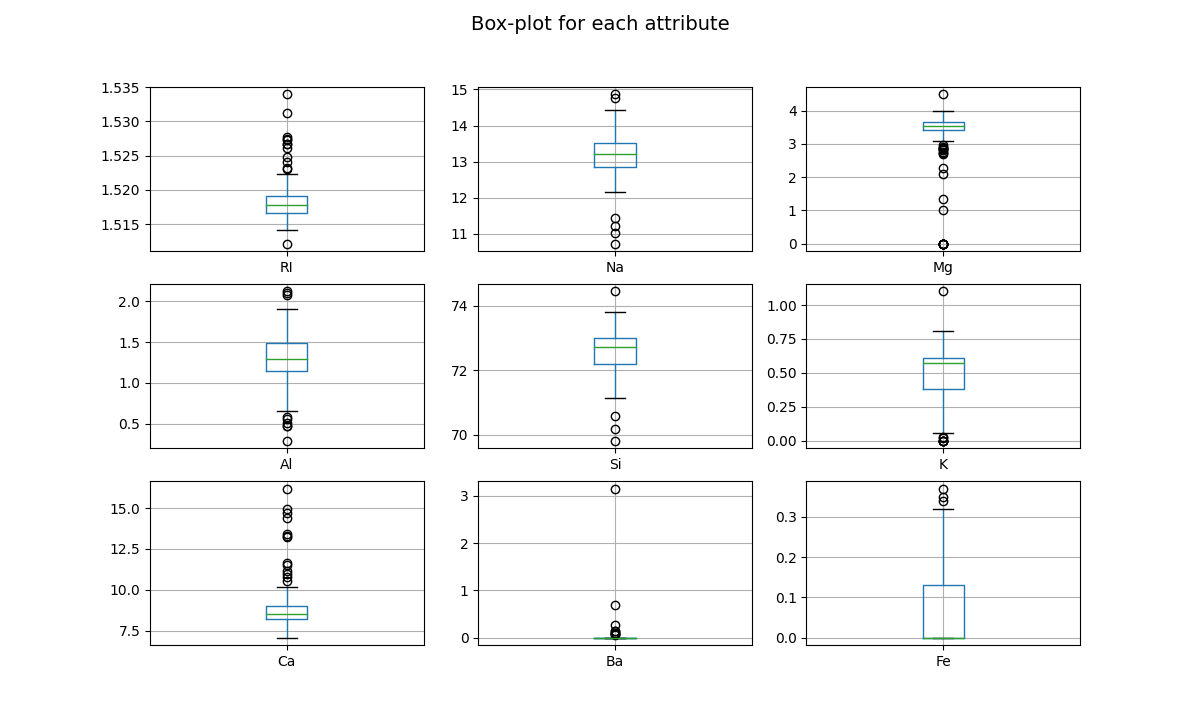
\includegraphics[width=\linewidth]{image/box-plot__for_each_attribute.png}
    	\caption{The attributes are visualized using a box-plot.}
    	\label{fig:box_plot}
    \end{figure}
We preferred to plot each attribute's box plot separately due to the values range discrepancy. Because of the raw values' physical meaning, we decided not to standardize the data for these analyses.
    
    \begin{figure}[H]
        \centering
    	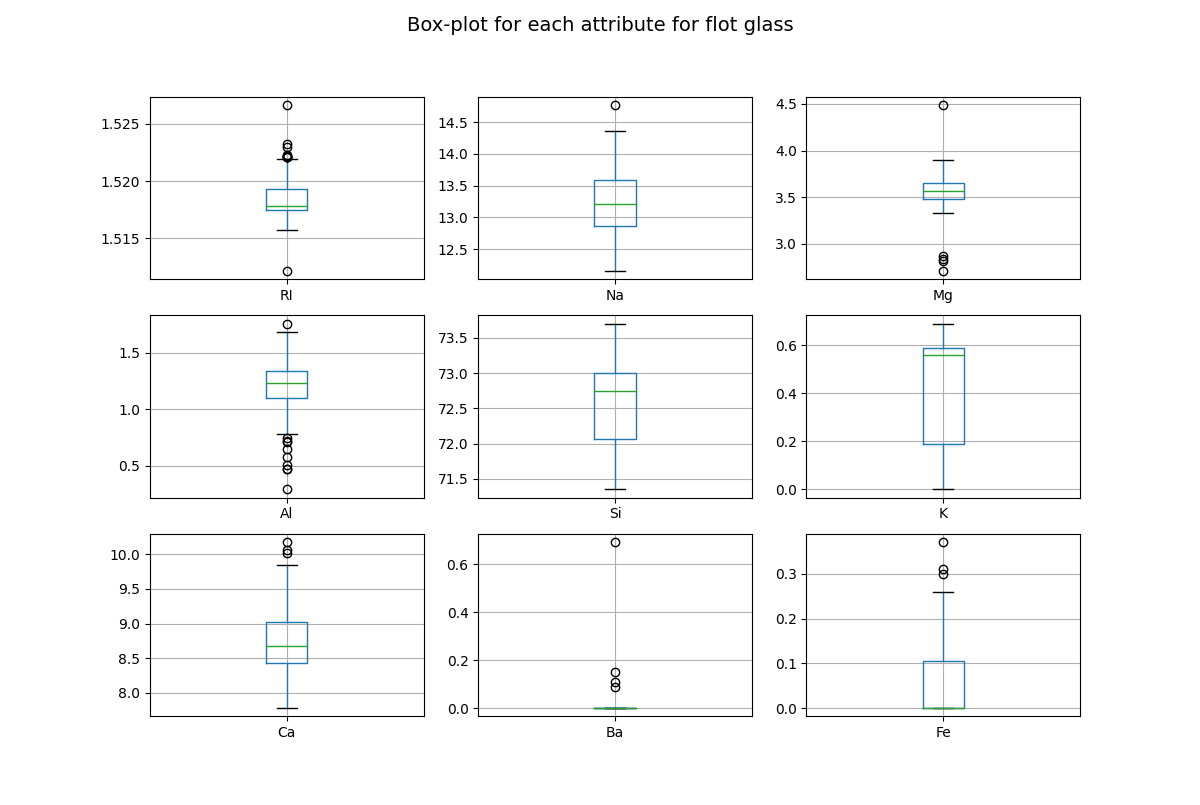
\includegraphics[width=\linewidth]{image/box-plot__for_each_attribute_for_float.png}
    	\caption{The attributes are visualized using a box-plot.}
    	\label{fig:box_plot_float}
    \end{figure}
    
    \begin{figure}[H]
        \centering
    	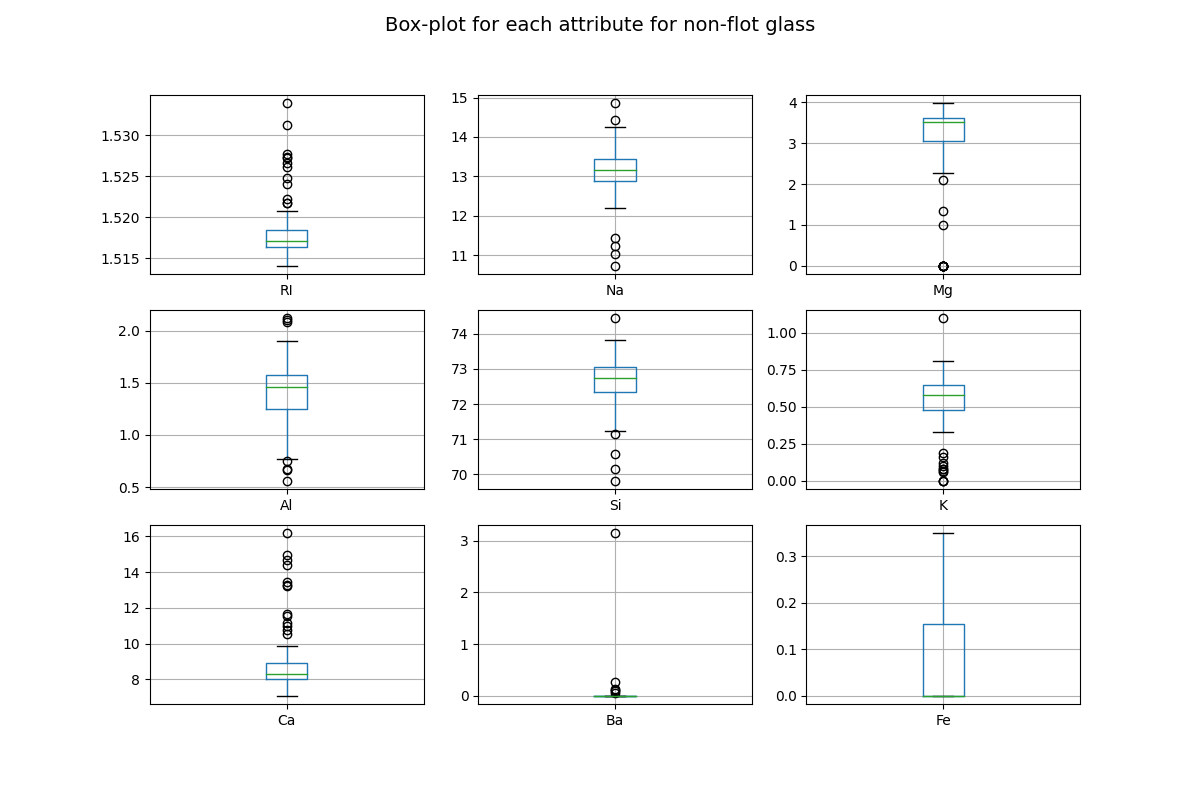
\includegraphics[width=\linewidth]{image/box-plot__for_each_attribute_for_non-float.png}
    	\caption{The attributes are visualized using a box-plot.}
    	\label{fig:box_plot_non_float}
    \end{figure}
    
To have a 2D view of the data, we created a scatter plot (Figure \ref{fig:scatter}) with each attribute against each other. The number of nine attributes is too large to have a relevant analysis. Hence, we choose to create a plot for $Na$, $Mg$, $Si$ and $Ca$ since they have the higher values for the standard deviation. The four attributes give us the greatest variance.
    
    \begin{figure}[H]
        \centering
    	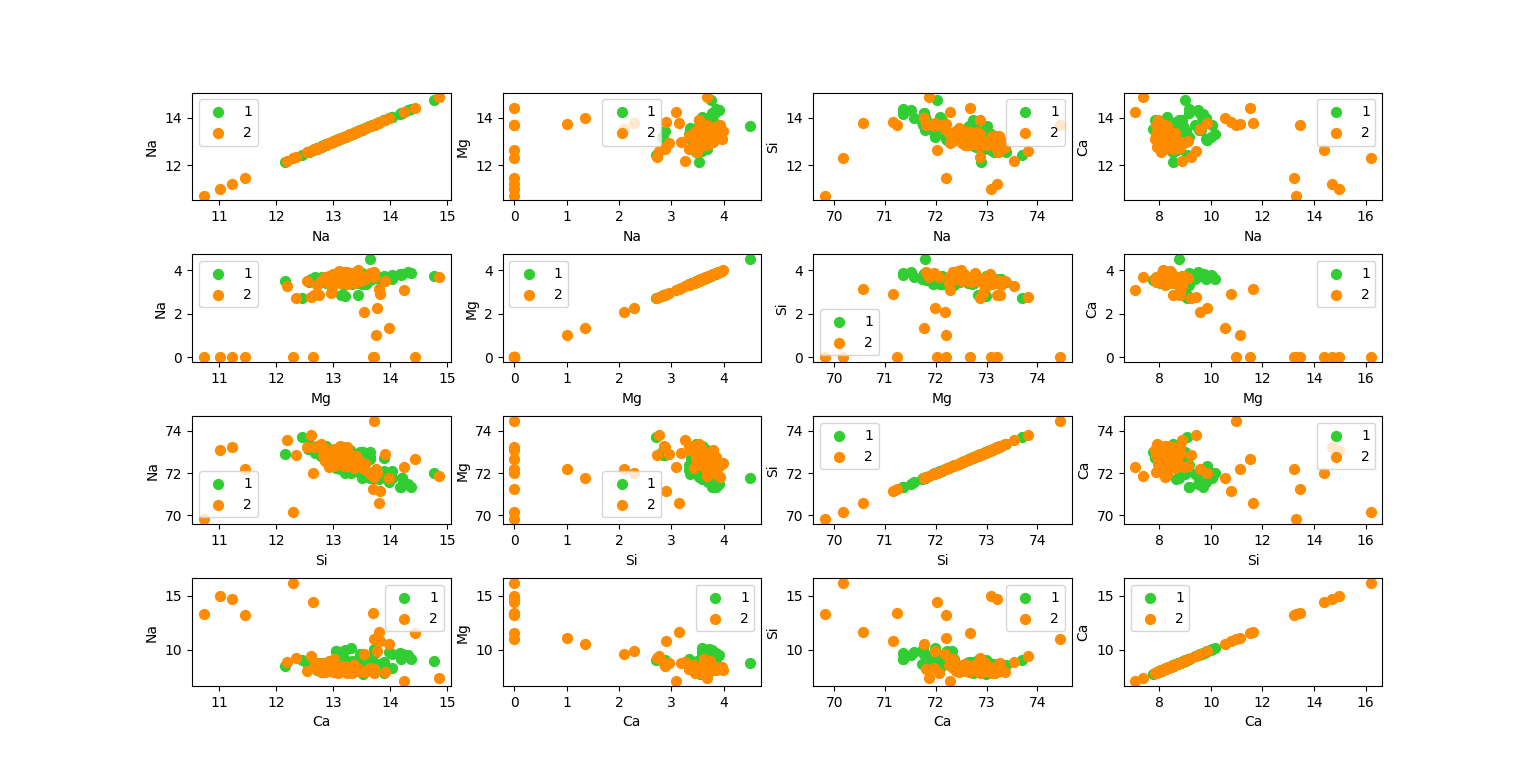
\includegraphics[width=\linewidth]{image/scatter_plot.png}
    	\caption{A matrix of scatter plots of each combination of two attributes against each other}
    	\label{fig:scatter}
    \end{figure}
After plotting the scatter plot for each attribute of the four, we noticed that it is difficult to discriminate between the two types of glass. Using only two attributes, we do not have the maximum variance. In the Figure \ref{fig:scatter} can be seen how the two classes overlaps most of the time. On the other hand, the plot give visual information about how the four attributes correlate, $Na$ and $Si$ correlate negatively, as and $Ca$ and $Si$. These observations are also validated by the correlation matrix (Figure \ref{fig:correlation_matrix}).
    

\section{Principal Component Analysis} \label{PCA}

Principal Component Analysis (PCA) will help us visualize and better understand our data set. The data set's main Machine Learning task is classification by glass types, with the data set having 7 glass types. The glass types and number of observations are show in Table \ref{table:4} below:

\begin{table}[H]
\begin{tabular}{|l|c|}
\hline
Glass Type                           & Number of observations \\ \hline
Float Processed Building Windows     & 70                     \\ \hline
Float Processed Vehicle Windows      & 17                     \\ \hline
Non-Float Processed Building Windows & 76                     \\ \hline
Non-Float Processed Vehicle Windows  & 0                      \\ \hline
Containers                           & 13                     \\ \hline
Tableware                            & 9                      \\ \hline
Headlamps                            & 29                     \\ \hline
\end{tabular}
\caption{Number of occurrences of each class.}
\label{table:4}
\end{table}

As it can be seen the classes are not equally distributed, so we decided that the main task of classification by type will be done between Float Processed glass, represented by class "1", and Non-Float Processed glass represented by class "2", thus we obtained a more uniform distribution between the two classes, with 87 observations for the first glass type and 76 observations for the second one. The obtained data set has a total of 163 observations from the original 214.

In the Figure \ref{fig:explained_var} the amount of explained variation as a number of principal components (PCs) included is shown. 

    \begin{figure}[H]
        \centering
    	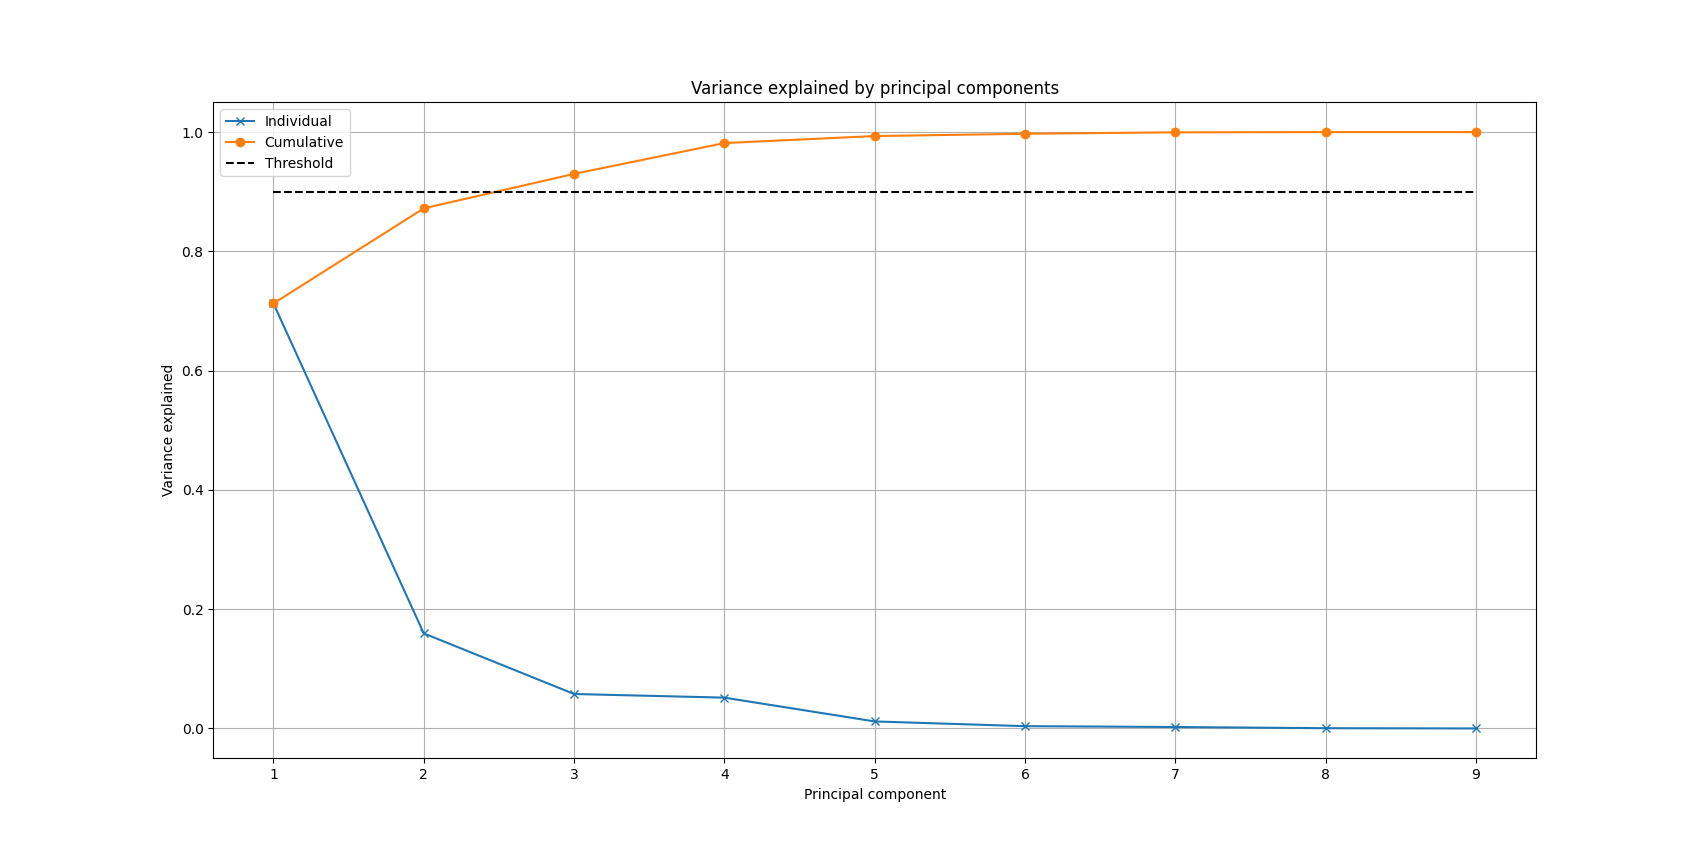
\includegraphics[width=\linewidth]{image/explained_variance.png}
    	\caption{Individual and cumulative explained variance as a function of principal components included.}
    	\label{fig:explained_var}
    \end{figure}

As it can be seen in the figure above more than $90\%$ of the variance is explained by the first three principal components, with the first four having a contribution of $5\%$ or above to the explained variance and explaining $98\%$ of the variance. Thus we can represent the data quite accurately using just 4 principal components instead of 9 features or PCs.

We also plotted the directions of the first three principal components by way of visualizing how much each feature contributes to the first three PCs.

    \begin{figure}[H]
        \centering
    	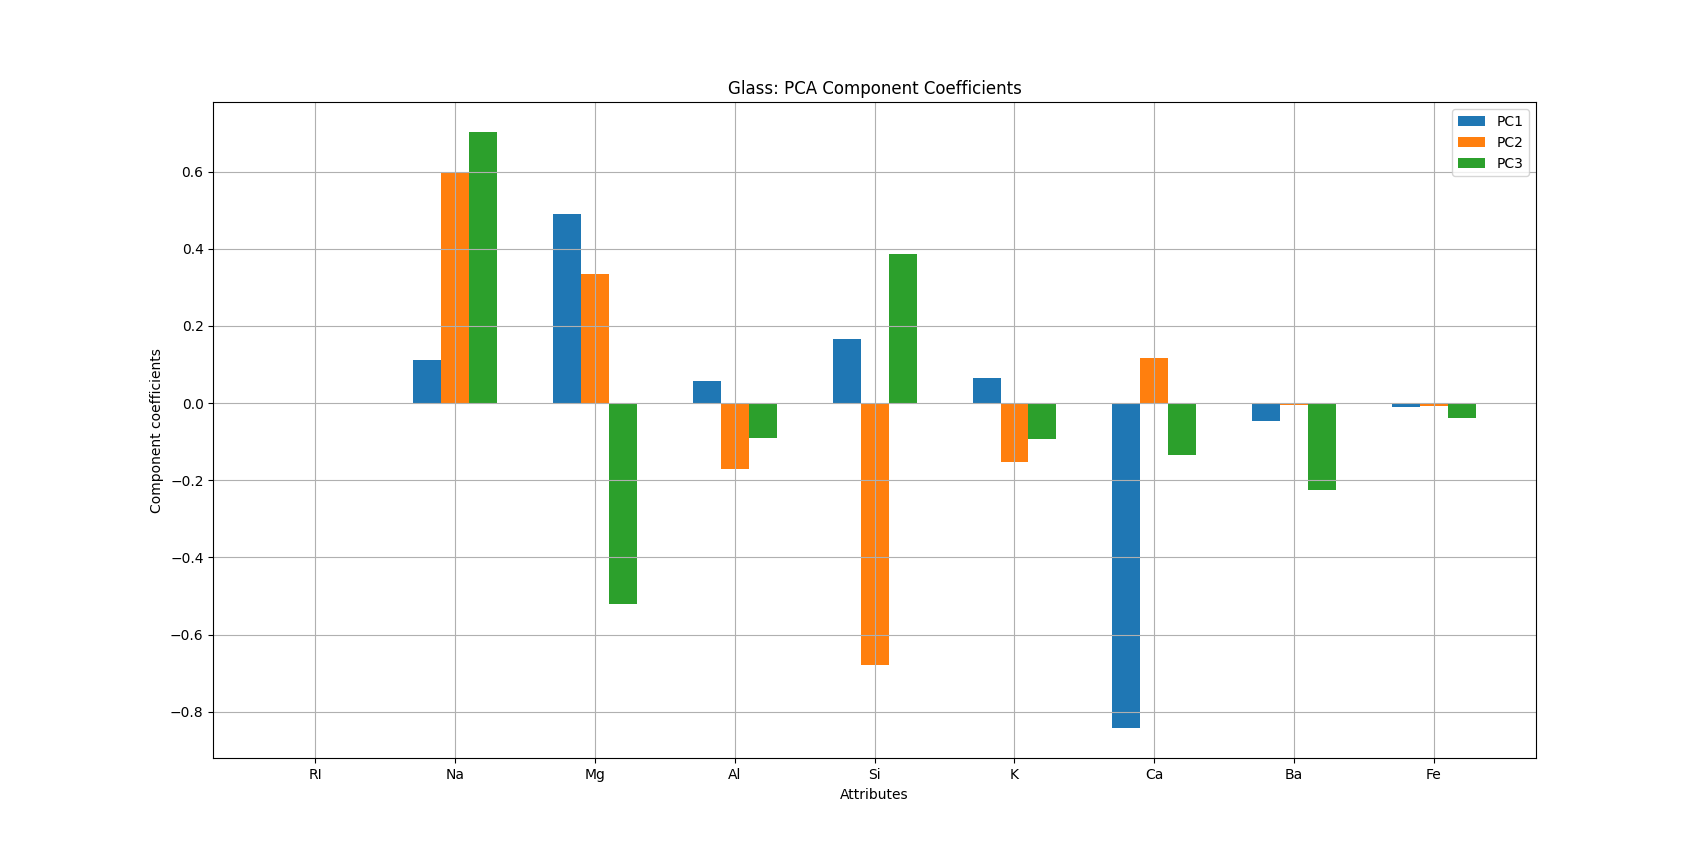
\includegraphics[width=\linewidth]{image/features_PCs.png}
    	\caption{How much each feature contributes to each of the first three PCs.}
    	\label{fig:features_PCs}
    \end{figure}
    
As it can be seen in Figure \ref{fig:features_PCs}, the refractive index contributes with almost nothing to the first three PCs, this may be due to it's very low standard deviation. Furthermore, it can be observed that Calcium and Magnesium attributes mainly contribute to the first PC. Silicon, Sodium and Magnesium are the main directions of the second PC, with the same three being the main contributors to the third PC. 

If we have a high value of Magnesium and a low value of Calcium we get a positive valued projection upon the first principal component and a negative valued projection if the values are reversed. We get a positive valued projection upon the second principal component if we have high values for Sodium and Magnesium, and low values of Silicon. 

The projection of the data set upon the first two principal components can be seen in Figure \ref{fig:projection_2PCs}.

    \begin{figure}[H]
        \centering
    	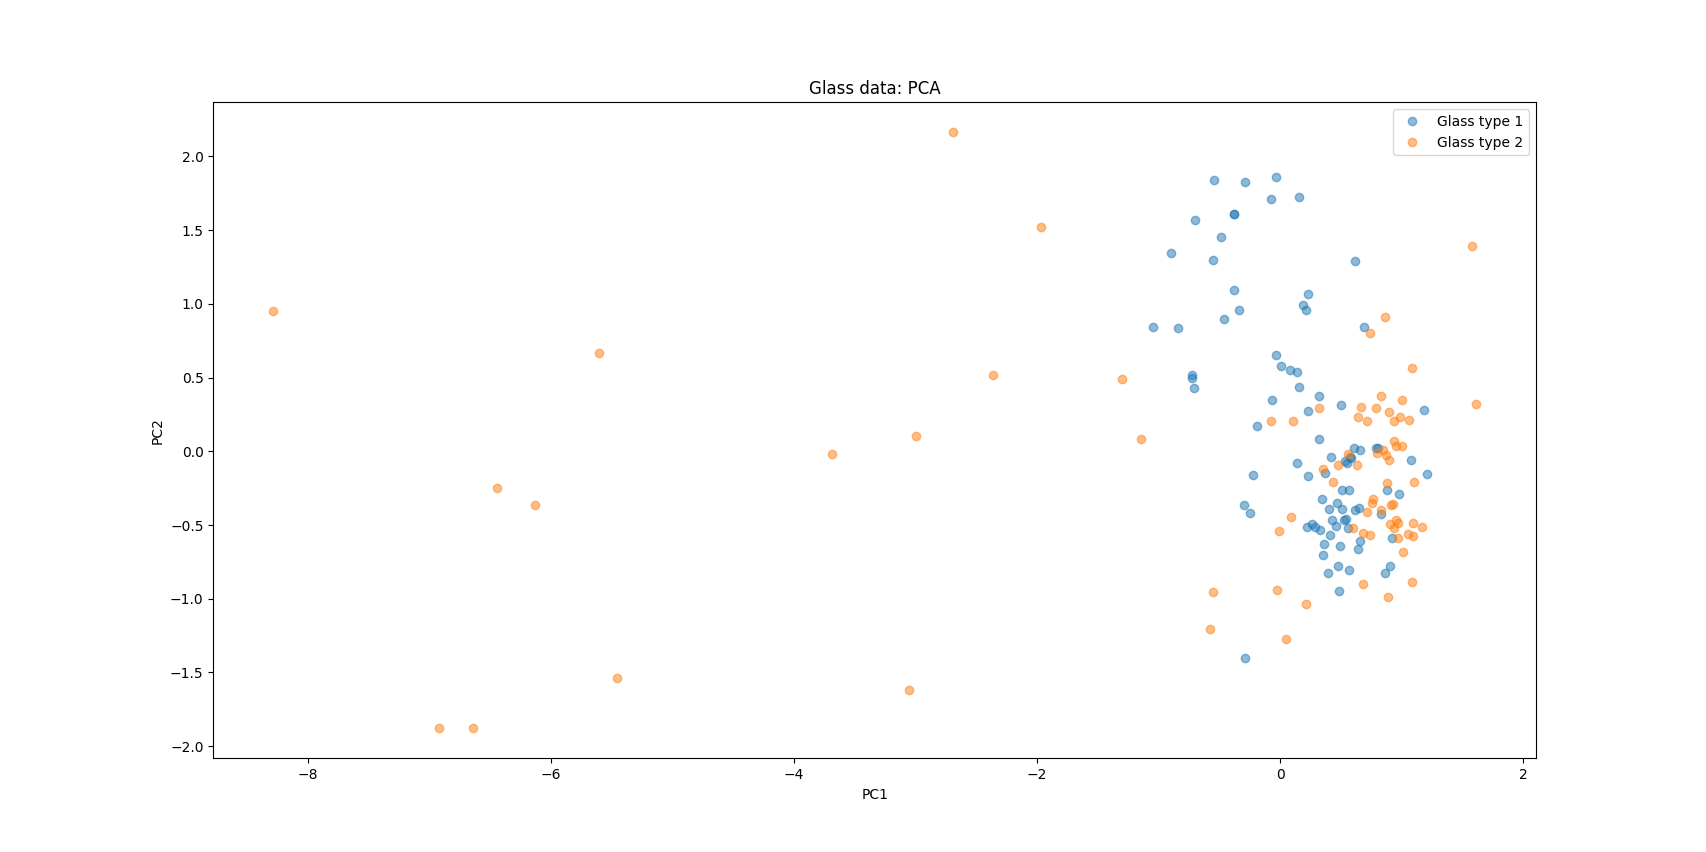
\includegraphics[width=\linewidth]{image/projection_2PCs.png}
    	\caption{Projecting the data set upon the first two principal components.}
    	\label{fig:projection_2PCs}
    \end{figure}
    
As it can be seen the second glass type, that is the Non-Float Processed glass, has a lot more variance than the Float Processed glass. This is rather interesting since the first glass type is composed of two sub-types of glass: Building Windows and Vehicle Windows, and we were expecting for this class to have more variance. 

Another important thing to notice from Figure \ref{fig:projection_2PCs} is that the two classes cannot be really separated by just using the first two principal components. 

\bibliography{references}
\newpage

% \appendix
\begin{appendices}
\section{Source code - GitHub}

The entire source code used for this project can be found using the following link: \url{https://github.com/fmazilu/Intro_ML_projects}
\end{appendices}

\end{document}
